\section{Actividad 03: Ejercicios de Calculos} 

\begin{enumerate}[1.]
    \item En Power BI Desktop, haga clic en Data en el panel de vistas en el lado izquierdo.

    \item En el panel Fields, haga clic en DimCustomer.

    \item En la cinta Modeling, en el grupo Calculations, haga clic en New Column.
    \item En la barra de fórmulas, resalte Column = y escriba:\\

	\begin{center}
	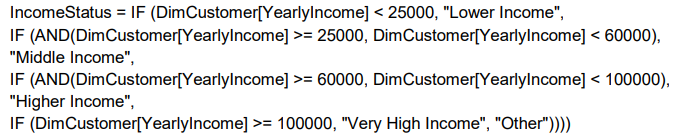
\includegraphics[width=13cm]{./Imagenes/code}
	\end{center}	

	\begin{center}
	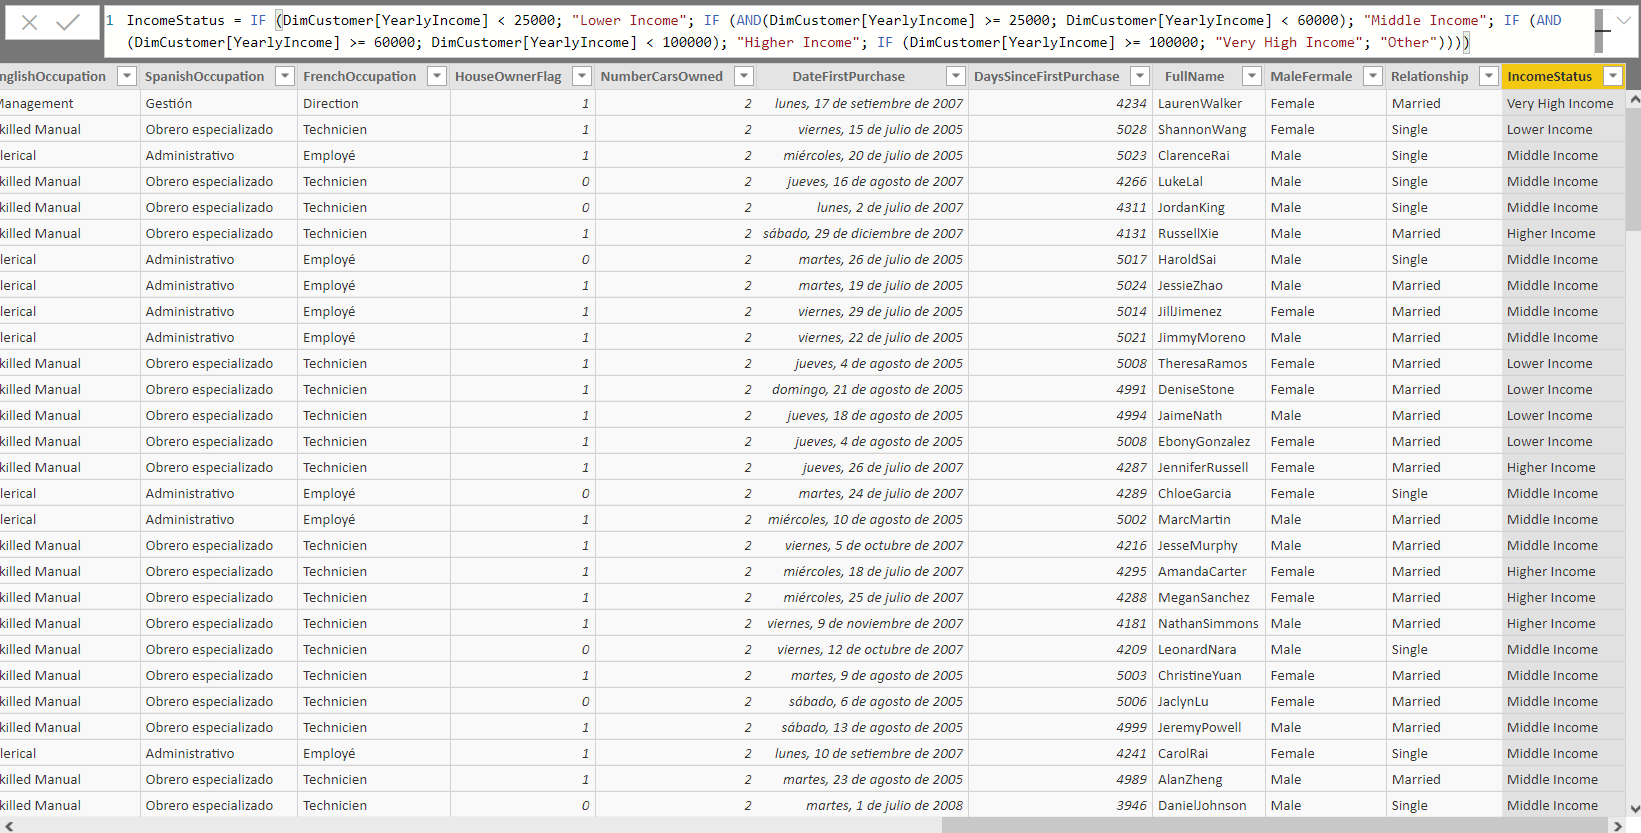
\includegraphics[width=18cm]{./Imagenes/power10}
	\end{center}	

    \item Presione Enter.
    \item En la cinta Modeling, en el grupo Calculations, haga clic en New Column.
    \item En la barra de fórmulas, resalte Column = y escriba: \\

\textbf{DaysSinceFirstPurchase = DATEDIFF(DimCustomer[DateFirstPurchase], TODAY(), DAY)}

	\begin{center}
	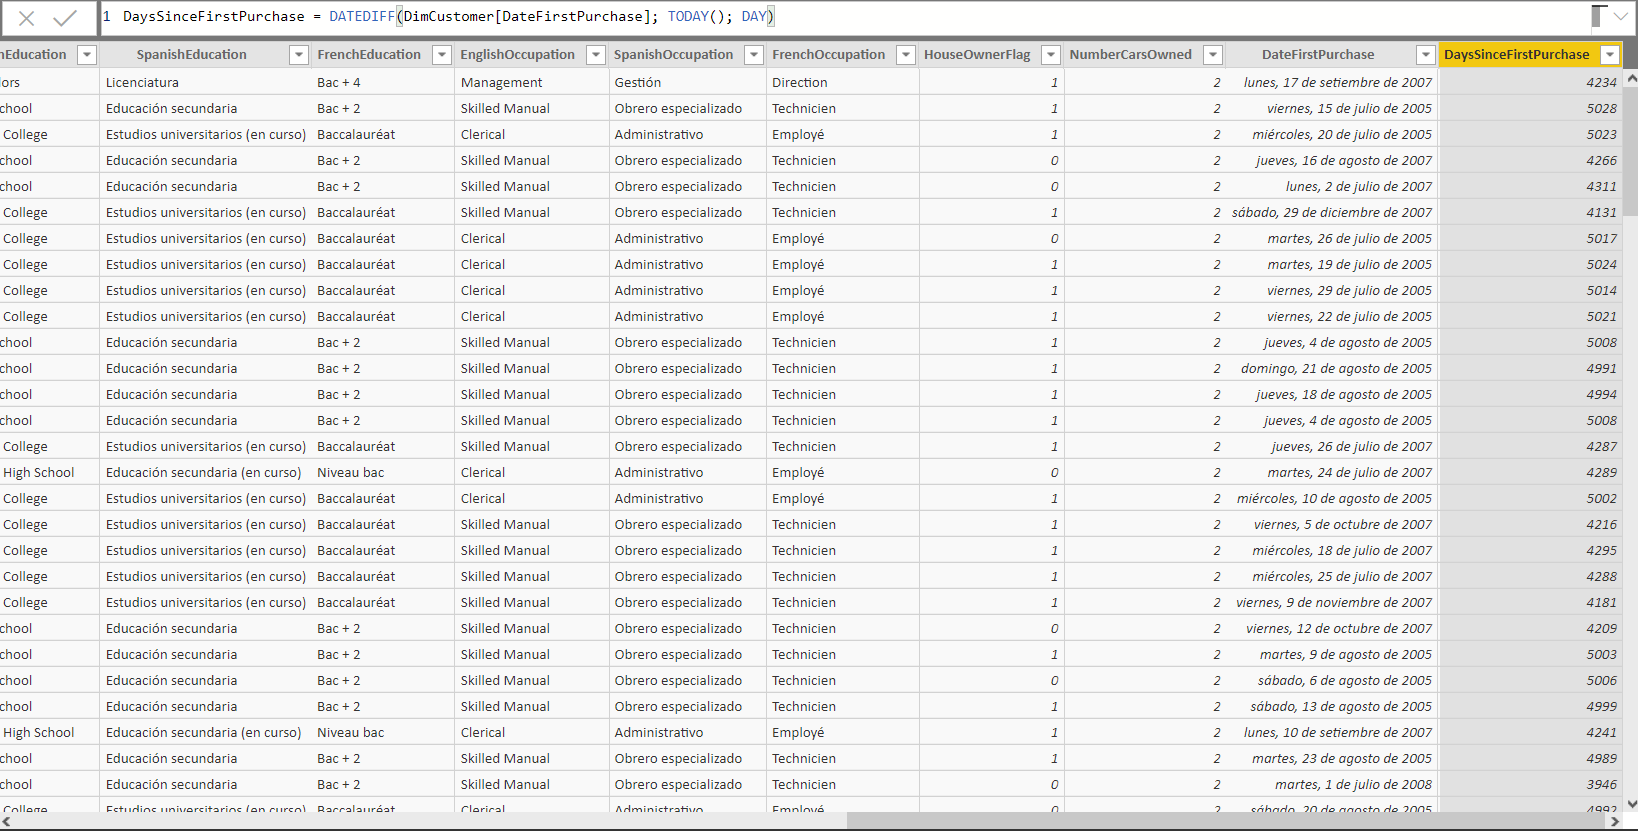
\includegraphics[width=18cm]{./Imagenes/power11}
	\end{center}	

    \item Presione Enter.

    \item En la cinta Modeling, en el grupo Calculations, haga clic en New Column.

    \item En la barra de fórmulas, resalte Column = y escriba: \\

\textbf{FullName = [FirstName] \& " " \& [LastName]}

	\begin{center}
	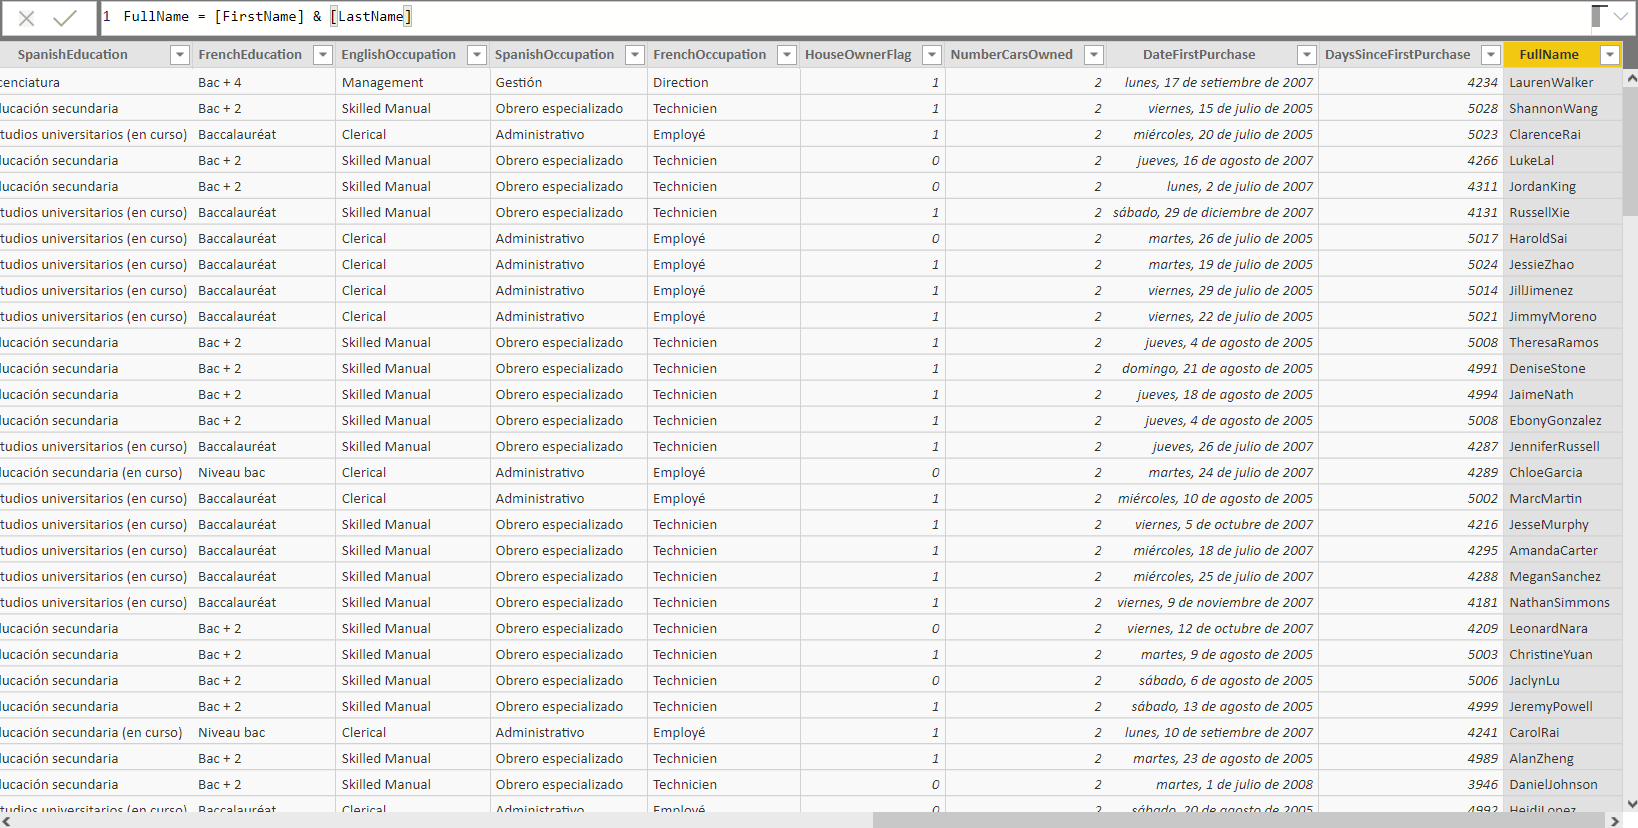
\includegraphics[width=18cm]{./Imagenes/power12}
	\end{center}	

    \item Presione Enter.
    \item En la cinta Modeling, en el grupo Calculations, haga clic en New Column.
    \item En la barra de fórmulas, resalte Column = y escriba: \\

\textbf{MaleFemale = IF([Gender] = "M", "Male", "Female")}

	\begin{center}
	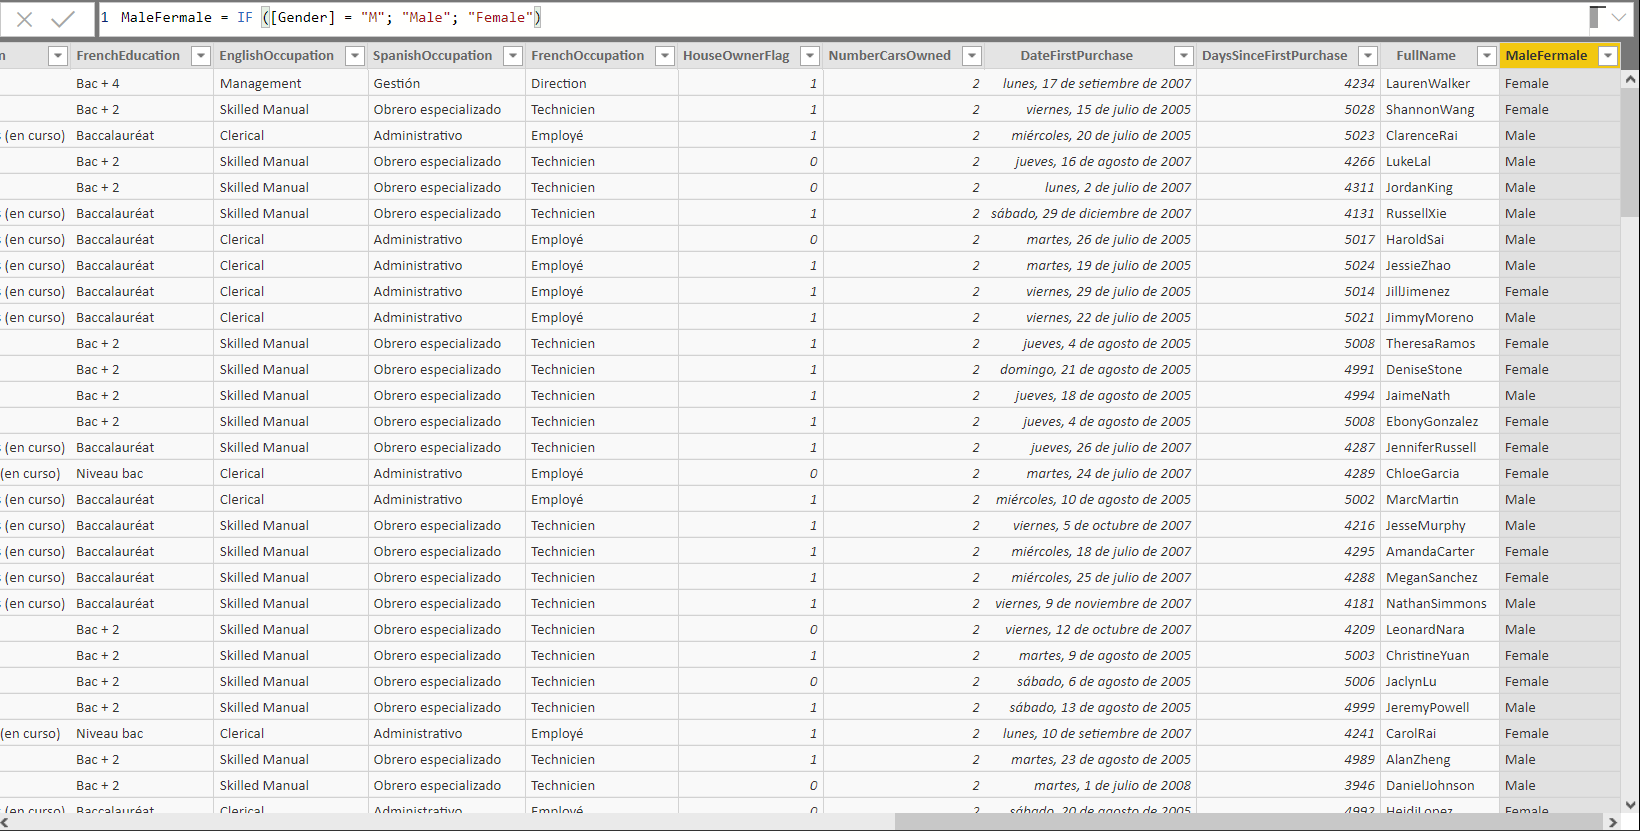
\includegraphics[width=18cm]{./Imagenes/power13}
	\end{center}	


    \item Presione Enter.
    \item En la cinta Modeling, en el grupo Calculations, haga clic en New Column.
    \item En la barra de fórmulas, resalte Column = y escriba:\\

\textbf{Relationship = IF([MaritalStatus] = "M", "Married", "Single")}

	\begin{center}
	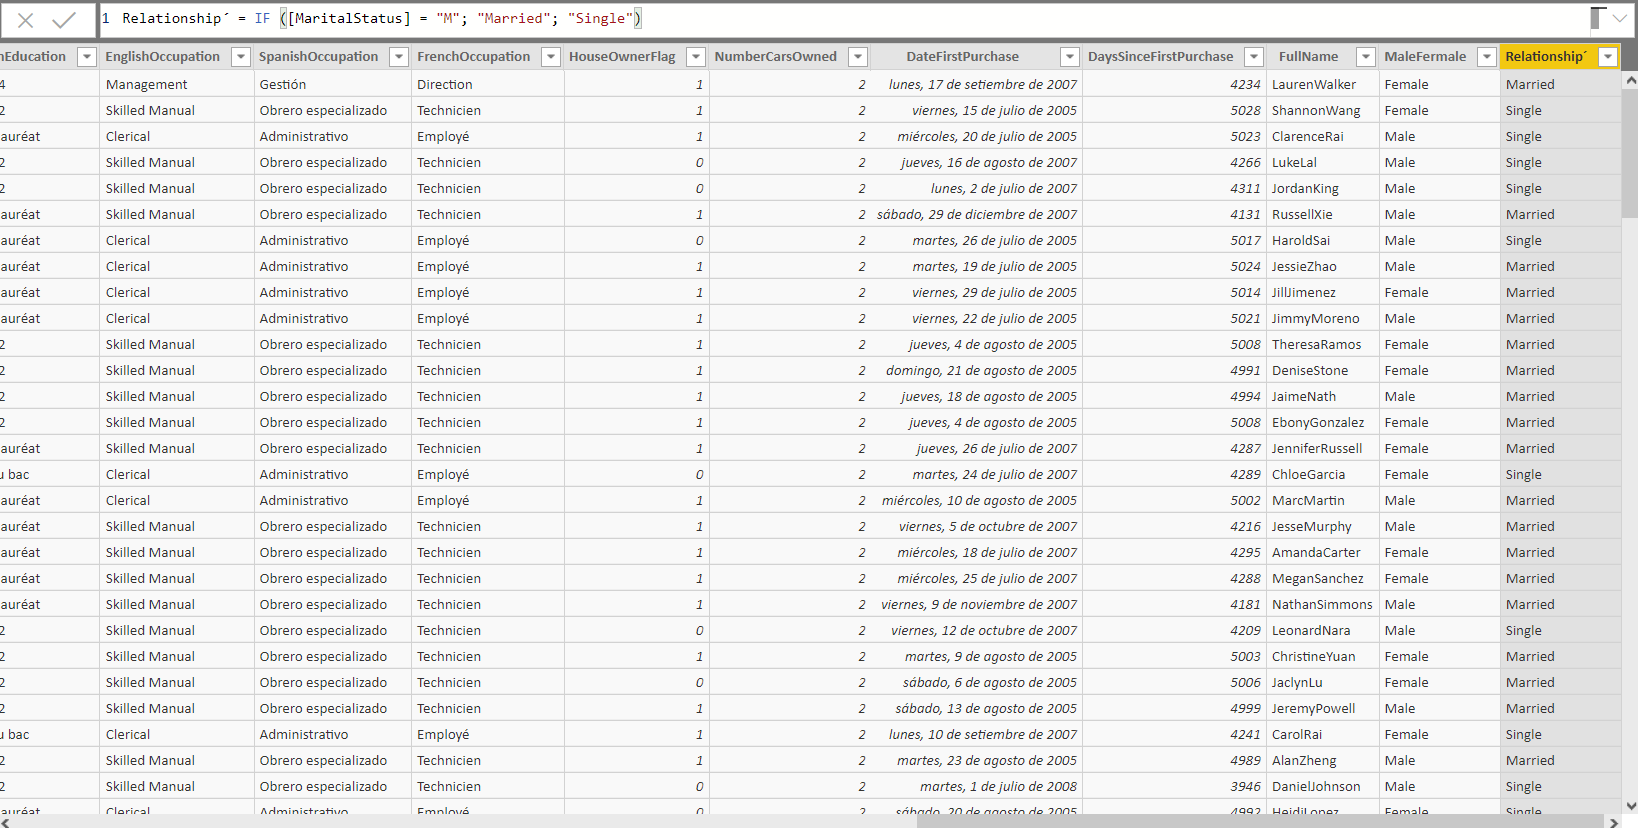
\includegraphics[width=18cm]{./Imagenes/power14}
	\end{center}	

    \item Presione Enter.
    \item En el panel Fields, haga clic en DimProductSubcategory.
    \item En la cinta de Modeling, en el grupo Calculations, haga clic en New Column.
    \item En la barra de fórmulas, resalte Column = y escriba: \\

\textbf{MainCategory = RELATED(DimProductCategory[CategoryName])}

	\begin{center}
	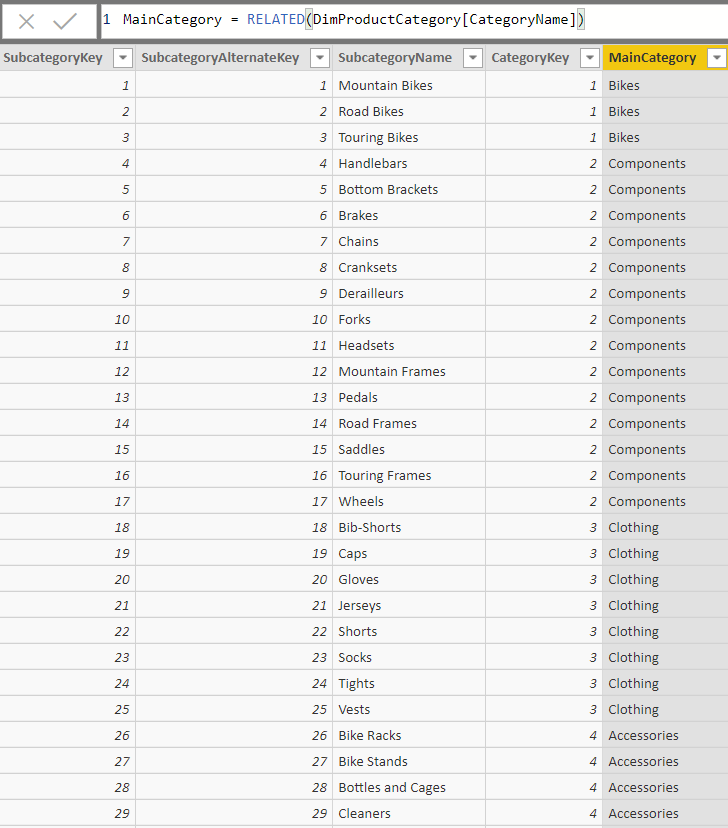
\includegraphics[width=13cm]{./Imagenes/power15}
	\end{center}	

    \item Presione Enter.
    \item En el panel Fields, haga clic en DimPromotion.
    \item En la cinta Modeling, en el grupo Calculations, haga clic en New Column.
    \item En la barra de fórmulas, resalte Column = y escriba: \\

\textbf{PromotionLengthDays = DATEDIFF(DimPromotion[StartDate],\\
DimPromotion[EndDate], DAY)}

	\begin{center}
	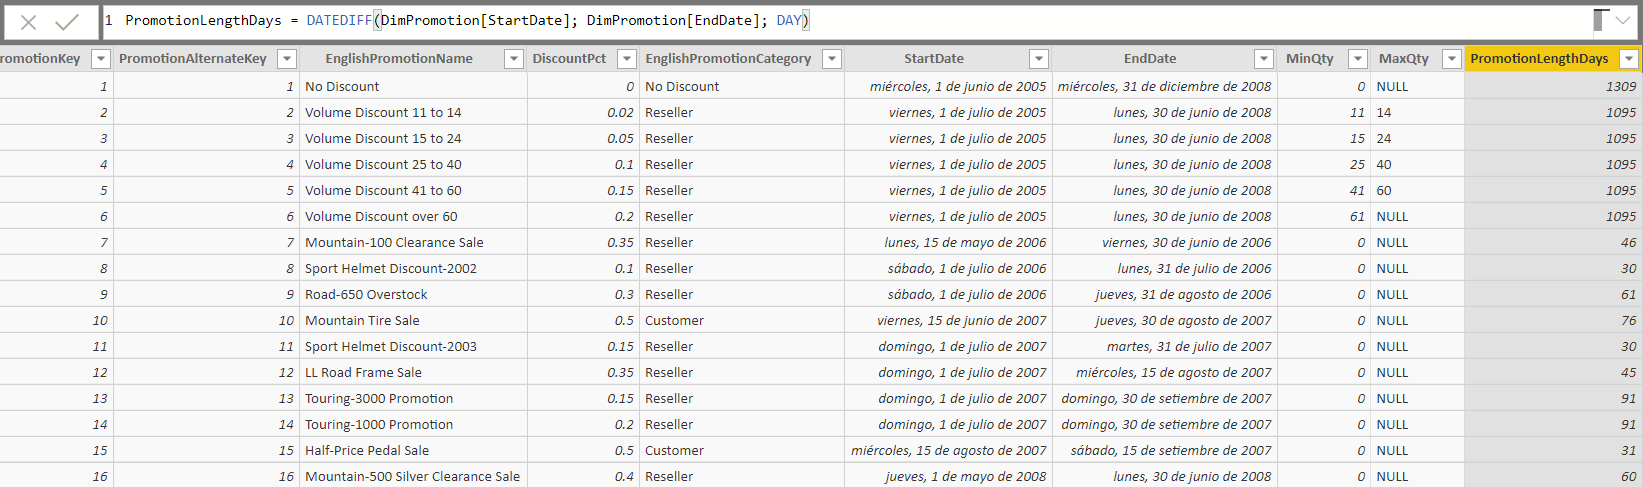
\includegraphics[width=18cm]{./Imagenes/power16}
	\end{center}	

    \item Presione Enter.
    \item En el panel Fields, haga clic en FactInternetSales.
    \item En la cinta Modeling, en el grupo Calculations, haga clic en New Column.
    \item En la barra de fórmulas, resalte Column = y escriba: \\

\textbf{Profit = CURRENCY(FactInternetSales[UnitPrice] - \\
FactInternetSales [ProductStandardCost])}

	\begin{center}
	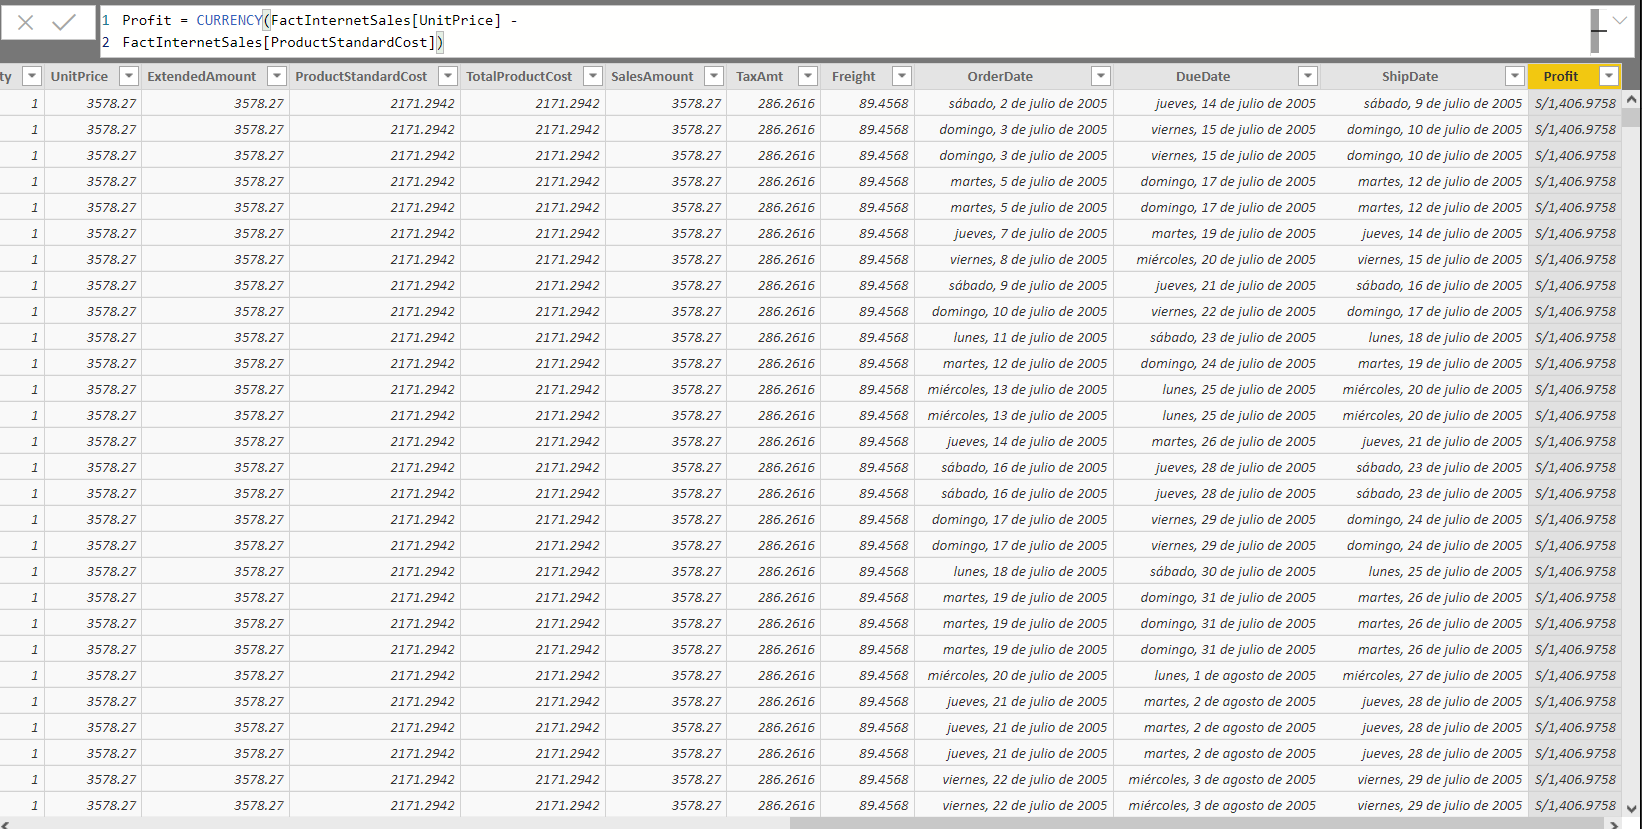
\includegraphics[width=18cm]{./Imagenes/power17}
	\end{center}	

    \item Presionar Enter.
    \item Cerrar Power BI Desktop, salvando cualquier cambio

\end{enumerate}